\documentclass[tikz,border=6mm]{standalone}
\usepackage{tikz}
\usepackage{xcolor}
\usetikzlibrary{arrows.meta,calc,decorations.pathmorphing,decorations.markings,shapes.geometric,positioning,backgrounds,fit,shadings,patterns}
\definecolor{substblue}{RGB}{70,130,180}
\definecolor{procamber}{RGB}{180,110,30}
\definecolor{feltgreen}{RGB}{0,110,55}
\definecolor{bgcream}{RGB}{252,248,240}
\definecolor{atomblue}{RGB}{100,160,210}
\definecolor{emphred}{RGB}{160,40,40}
\definecolor{panelborder}{RGB}{180,170,155}

\begin{document}
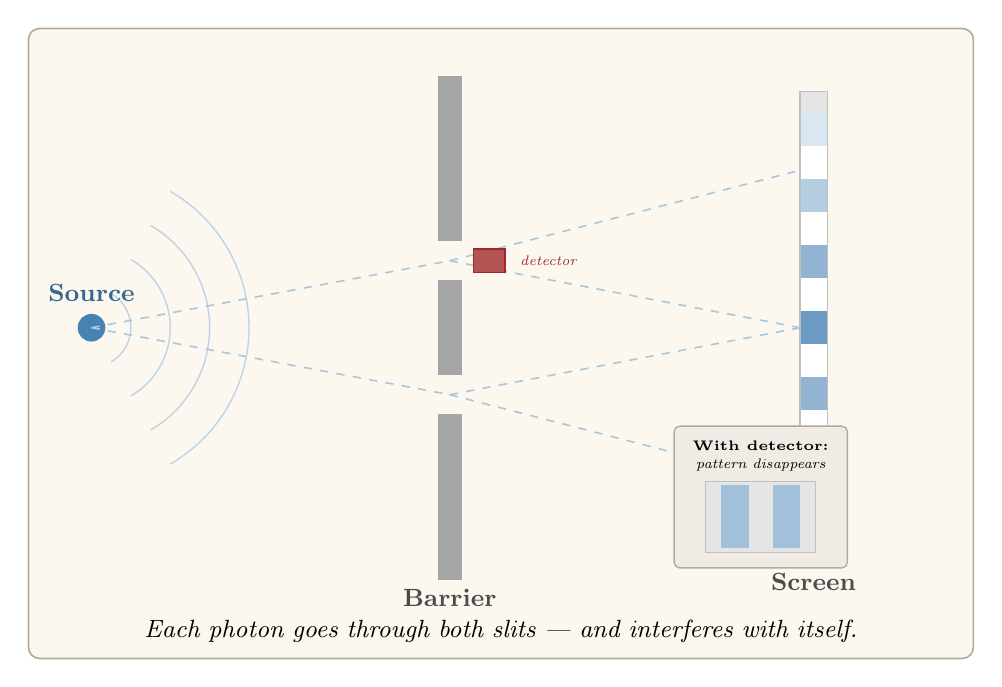
\begin{tikzpicture}[>=Stealth]

%% ── background ──────────────────────────────────────────────────────────────
\fill[bgcream,rounded corners=4pt] (-0.8,-4.2) rectangle (11.2,3.8);
\draw[panelborder,rounded corners=4pt,line width=0.6pt]
  (-0.8,-4.2) rectangle (11.2,3.8);

%% ── concentric wave arcs from source ────────────────────────────────────────
\foreach \r in {0.5,1.0,1.5,2.0}{%
  \draw[substblue!35,line width=0.5pt]
    (0,0) ++(-60:\r) arc[start angle=-60,end angle=60,radius=\r];
}

%% ── source dot ──────────────────────────────────────────────────────────────
\fill[substblue] (0,0) circle (5pt);
\node[above=6pt,font=\small\bfseries,substblue!80!black] at (0,0) {Source};

%% ── barrier ─────────────────────────────────────────────────────────────────
% solid sections
\fill[gray!70] (4.4,-3.2) rectangle (4.7,-1.1);  % bottom solid
\fill[gray!70] (4.4,-0.6) rectangle (4.7, 0.6);  % middle solid (between slits)
\fill[gray!70] (4.4, 1.1) rectangle (4.7, 3.2);  % top solid
\node[below,font=\small\bfseries,gray!60!black] at (4.55,-3.2) {Barrier};

%% ── wave paths through slits (dashed) ───────────────────────────────────────
% upper slit centre ~ y=0.85
\draw[substblue!45,dashed,line width=0.6pt]
  (0,0) -- (4.55, 0.85);
\draw[substblue!45,dashed,line width=0.6pt]
  (4.55, 0.85) -- (9.0, 0.0);
\draw[substblue!45,dashed,line width=0.6pt]
  (4.55, 0.85) -- (9.0, 2.0);
% lower slit centre ~ y=-0.85
\draw[substblue!45,dashed,line width=0.6pt]
  (0,0) -- (4.55,-0.85);
\draw[substblue!45,dashed,line width=0.6pt]
  (4.55,-0.85) -- (9.0, 0.0);
\draw[substblue!45,dashed,line width=0.6pt]
  (4.55,-0.85) -- (9.0,-2.0);

%% ── screen base ─────────────────────────────────────────────────────────────
\fill[gray!20] (9.0,-3.0) rectangle (9.35,3.0);
\draw[gray!50,line width=0.5pt] (9.0,-3.0) rectangle (9.35,3.0);
\node[below,font=\small\bfseries,gray!60!black] at (9.17,-3.0) {Screen};

%% ── interference fringes (bright/dark bands) on screen ─────────────────────
% Bands centred on y=0; each band height = 0.42cm.
% centre (brightest) then alternating dark/bright outward
\pgfmathsetmacro{\bw}{0.42}
% centre bright
\fill[substblue!80] (9.0,-\bw/2) rectangle (9.35,\bw/2);
% 1st pair
\fill[white]         (9.0, \bw/2)   rectangle (9.35,{1.5*\bw});
\fill[white]         (9.0,-\bw/2)   rectangle (9.35,{-1.5*\bw});
\fill[substblue!60] (9.0,{1.5*\bw}) rectangle (9.35,{2.5*\bw});
\fill[substblue!60] (9.0,{-1.5*\bw}) rectangle (9.35,{-2.5*\bw});
% 2nd pair
\fill[white]         (9.0,{2.5*\bw}) rectangle (9.35,{3.5*\bw});
\fill[white]         (9.0,{-2.5*\bw}) rectangle (9.35,{-3.5*\bw});
\fill[substblue!40] (9.0,{3.5*\bw}) rectangle (9.35,{4.5*\bw});
\fill[substblue!40] (9.0,{-3.5*\bw}) rectangle (9.35,{-4.5*\bw});
% 3rd pair (faint)
\fill[white]         (9.0,{4.5*\bw}) rectangle (9.35,{5.5*\bw});
\fill[white]         (9.0,{-4.5*\bw}) rectangle (9.35,{-5.5*\bw});
\fill[substblue!20] (9.0,{5.5*\bw}) rectangle (9.35,{6.5*\bw});
\fill[substblue!20] (9.0,{-5.5*\bw}) rectangle (9.35,{-6.5*\bw});
% redraw screen border on top
\draw[gray!50,line width=0.5pt] (9.0,-3.0) rectangle (9.35,3.0);

%% ── detector icon at upper slit ─────────────────────────────────────────────
\fill[emphred!80] (4.85,0.7) rectangle (5.25,1.0);
\draw[emphred,line width=0.5pt] (4.85,0.7) rectangle (5.25,1.0);
\node[right=2pt,font=\tiny\itshape,emphred] at (5.25,0.85) {detector};

%% ── inset: "with detector → classical pattern" ───────────────────────────────
\begin{scope}[shift={(7.5,-2.2)}]
  \fill[bgcream!90!gray,rounded corners=2pt] (-0.1,-0.85) rectangle (2.1,0.95);
  \draw[panelborder,rounded corners=2pt,line width=0.5pt]
    (-0.1,-0.85) rectangle (2.1,0.95);
  \node[font=\tiny\bfseries,align=center] at (1.0,0.70)
    {With detector:};
  \node[font=\tiny\itshape,align=center] at (1.0,0.45)
    {pattern disappears};
  % two classical bands
  \fill[gray!20]       (0.30,-0.65) rectangle (1.70, 0.25);
  \fill[substblue!50] (0.50,-0.60) rectangle (0.85, 0.20);
  \fill[substblue!50] (1.15,-0.60) rectangle (1.50, 0.20);
  \draw[gray!50,line width=0.4pt] (0.30,-0.65) rectangle (1.70, 0.25);
\end{scope}

%% ── figure caption (below Barrier/Screen labels) ────────────────────────────
\node[font=\small\itshape,text width=10cm,align=center]
  at (5.2,-3.85)
  {Each photon goes through both slits --- and interferes with itself.};

\end{tikzpicture}
\end{document}
